
\begin{figure}[H]
	\centering
	\begin{minipage}[b]{0.49\textwidth}
		(a)
		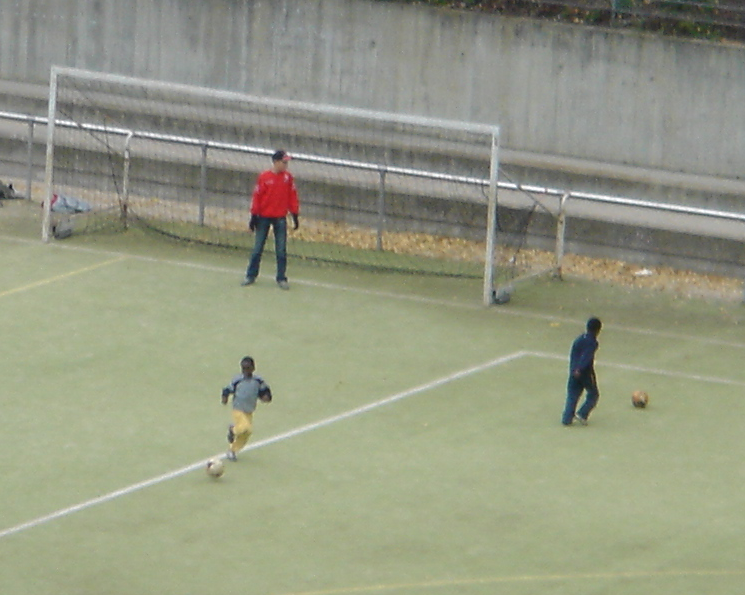
\includegraphics[width=0.94\textwidth]{Bilder/hog1crop.png}
	\end{minipage}
	\hfill
	\begin{minipage}[b]{0.49\textwidth}
		(b)
		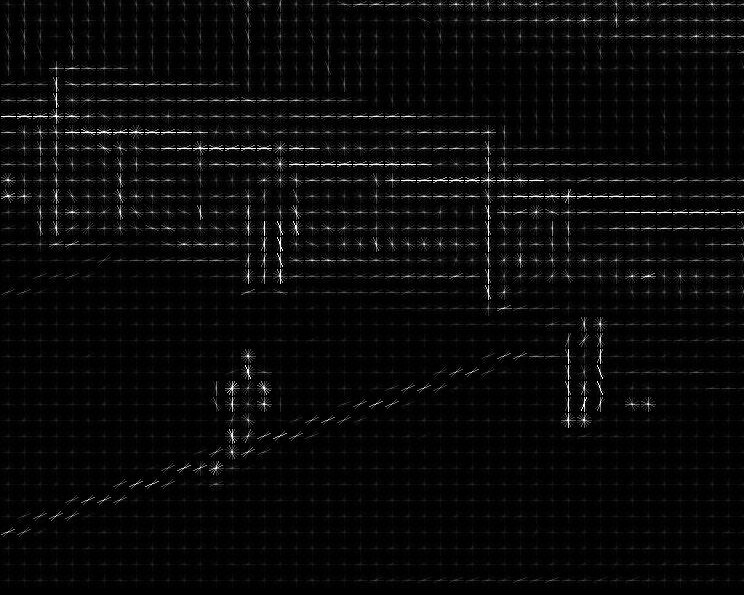
\includegraphics[width=0.94\textwidth]{Bilder/hog2crop.jpg}
	\end{minipage}
	\caption{(a) Foto von drei spielenden Personen \cite{inria1}. (b) Darstellung der Gradienten, die durch einen \textit{HOG} erzeugt worden sind. Der weiße Farbverlauf deutet die Richtung der analysierten Konturen an. Die Analyse erfolgte mit Bild a \cite{inria1}.}
	\label{fiq: hog}
\end{figure}
